%% Template para disserta????o/tese na classe UFBAthesis
%% versao 1.0
%% (c) 2005 Paulo G. S. Fonseca
%% (c) 2012 Antonio Terceiro
%% (c) 2014 Christina von Flach
%% www.dcc.ufba.br/~flach/ufbathesis

%% Carrega a classe ufbathesis
%% Opcoes: * Idiomas
%%           pt   - portugues (padrao)
%%           en   - ingles
%%         * Tipo do Texto
%%           bsc  - para monografias de graduacao
%%           msc  - para dissertacoes de mestrado (padrao)
%%           qual - exame de qualificacao de mestrado
%%           prop - exame de qualificacao de doutorado
%%           phd  - para teses de doutorado
%%         * M??dia
%%           scr  - para vers??o eletr??nica (PDF) / consulte o guia do usuario
%%         * Estilo
%%           classic - estilo original a la TAOCP (deprecated)
%%           std     - novo estilo a la CUP (padrao)
%%         * Paginacao
%%           oneside - para impressao em face unica
%%           twoside - para impressao em frente e verso (padrao)
\documentclass[bsc, classic, a4paper, twoside]{ufbathesis}
\usepackage[utf8]{inputenc}
\usepackage{indentfirst}
\usepackage{booktabs}
\usepackage{float}

\makeatletter  
\def\NAT@parse{\typeout{This is a fake Natbib command to fool Hyperref.}}  
\makeatother  

\usepackage{hyperref}
\usepackage{graphicx}

%% Preambulo:
%% coloque aqui o seu preambulo LaTeX, i.e., declara????o de pacotes,
%% (re)definicoes de macros, medidas, etc.

%% Identificacao:

% Universidade
\university{UNIVERSIDADE FEDERAL DA BAHIA}

% Endereco (cidade)
% e.g. \address{Campinas}
\address{Salvador}

% Instituto ou Centro Academico
% e.g. \institute{Centro de Ciencias Exatas e da Natureza}
% Comente se nao se aplicar
\institute{Departamento de Engenharia Elétrica e Computação}

% Nome da biblioteca - usado na ficha catalografica
% default: nome da biblioteca do Instituto de Matematica
\library{BIBLIOTECA REITOR MACÊDO COSTA}

% Programa de pos-graduacao
% e.g. \program{Pos-graduacao em Ciencia da Computacao}
\program{Departamento de Engenharia Elétrica e de Computação}

% ?rea de titulacao
\majorfield{Engenharia de Computação}

% Titulo da dissertacao/tese
% e.g. \title{Sobre a conjectura $P=NP$}
\title{Análise do tempo da latência de interrupção no Raspberry Pi em diferentes patches de tempo real para o kernel Linux}

% Data da defesa
% e.g. \date{19 de fevereiro de 2003}
\date{DIA de MÊS de ANO}

% Autor
% e.g. \author{Jose da Silva}
\author{Taian Fonseca Feitosa}

% Orientador(a)
% Opcao: [f] - para orientador do sexo feminino
% e.g. \adviser[f]{Profa. Dra. Maria Santos}
\adviser{Paul Regnier}

% Orientador(a)
% Opcao: [f] - para orientador do sexo feminino
% e.g. \coadviser{Prof. Dr. Pedro Pedreira}
% Comente se nao se aplicar
% \coadviser{NOME DO(DA) CO-ORIENTADOR(A)}

%% Inicio do documento
\begin{document}

\pgcompfrontpage{}

%%
%% Parte pre-textual
%%
\frontmatter

%\pgcomppresentationpage
% Se seu trabalho for uma disserta??o de mestrado do PGCOMP, use a linha acima
%\presentationpage
% Se for qualificacao, use \presentationpage

% Ficha catalogrofica
\authorcitationname{Feitosa, Taian Fonseca} % e.g. Terceiro, Antonio Soares de Azevedo
\advisercitationname{Regnier, Paul} % e.g. Chavez, Christina von Flach Garcia
%\coadvisercitationname{NOME DO SEU CO-ORIENTADOR EM CITACOES} % e.g. Mendonca, Manoel Gomes de
\catalogtype{Trabalho de Conclusão de Curso} % e.g. ``Tese (doutorado)''
\catalogtopics{1. Raspberry Pi. 2. Sistemas de tempo real. 3. PREEMPT-RT. 4. Drones. 5. Sistemas embarcados} % e.g. ``1. Complexidade Estrutural. 2. Engenharia de Software''
\catalogcdd{CDD 20.ed. XXX.YY} % e.g. ``CDD 20.ed. XXX.YY'' (esse n??mero vai lhe ser dado pela biblioteca)
\catalogingsheet

% Termo de aprovacaoo
% Se seu trabalho for Tese de Doutorado, inclua comitteemember 4 e 5
\approvalsheet{Salvador, DIA de MES de ANO}{
  \comittemember{Profa. Dra. Professora 1}{Universidade XYZ}
  \comittemember{Prof. Dr. Professor 2}{Universidade 123}
  \comittemember{Profa. Dra. Professora 3}{Universidade ABC}
%  \comittemember{Prof. Dr. Professor 4}{Universidade HJKL}
%  \comittemember{Profa. Dra. Professora 5}{Universidade QWERTY}
}

% Dedicatoria
% Comente para ocultar
\begin{dedicatory}
Dedicatória
\end{dedicatory}

% Agradecimentos
% Se preferir, crie um arquivo ?? parte e o inclua via \include{}
\acknowledgements
Agradecimentos

% Epigrafe
% Comente para ocultar
% e.g.
\begin{epigraph}[Um dia]{Eu mesmo}
Epígrafe
\end{epigraph}

% Resumo em Portugues
% Se preferir, crie um arquivo separado e o inclua via \include{}
\resumo
A popularização dos Veículos Aéreos Não Tripulados (VANTs), mais conhecidos como drones, trouxe praticidade e comodidade para executar várias tarefas que sem sua ajuda seriam muito trabalhosas ou mesmo muito perigosas. Segunda a ANAC, Agência Nacional de Aviação Civil, em julho de 2019 o Brasil já tinha mais de 70 mil drones cadastrados, sendo mais de 25 mil para uso profissional e mais de 45 mil para uso recreativo. Para algumas atividades mais simples o controle manual de um drone é suficiente mas para atividades mais extensivas ou repetitivas o controle manual não é apropriado. Alguns drones mais simples não possuem capacidade de adicionar mais sensores e uma alternativa comum é acoplar um sistema embarcado, como um Raspberry Pi, para controlar o drone através da API do fabricante do drone. Este sistema embarcado deve sempre ser capaz de responder dentro de um período crítico, pois um atraso na leitura do sensor ou no controle do drone, dependendo de sua aplicação, pode levar a falhas catastróficas e potencialmente colocar em risco a vida humana. Neste contexto, este trabalho tem como objetivo avaliar o tempo de resposta de Raspberry Pi 3 Modelo B, modelo utilizado no LaSiD - Laboratório de Sistemas Distribuídos para pesquisas com o drone AR.Drone 2.0 fabricado pela Parrot, em diferentes cenários e em diferentes implementações do kernel do linux, como o patch PREEMPT-RT, para ajudar os projetistas de aplicativos a desenvolver sistemas de controle de drones.

% Palavras-chave do resumo em Portugues
\begin{keywords}
Raspberry Pi; Sistemas de tempo real; PREEMPT-RT; Drones; Sistemas embarcados
\end{keywords}


% Resumo em Ingles
% Se preferir, crie um arquivo separado e o inclua via \include{}
\abstract
Modern computer systems are capable of performing many tasks and also need to meet a variety of requirements. Some systems have time requirements and need to respond quickly and correctly to external events such as cars, aircraft, robotic systems, and other mechatronic systems, where a delayed response may compromise system integrity. For this, specific operating systems are designed to meet these requirements, the real-time operating systems. These external events are signaled to the processor through the interrupt mechanism. To keep the system responsive, these interrupts need to be addressed in a short and predictable time. As systems are increasingly complex, accurate analysis models do not exist, so measurement strategies are the best way to verify system responsiveness. One of the most popular embedded systems is the Raspberry Pi, a small, low-cost, low-power platform that uses Linux, one of the most popular operating systems in the world. This makes Raspberry Pi one of the most widely used platforms for the development of embedded systems in various projects. This work analyzes Raspberry's latency when responding to external events on standard Linux and Preempt-RT, a realtime patch for Linux.

% Palavras-chave do resumo em Ingles
\begin{keywords}
Raspberry Pi; Real-time systems; Preempt-RT; Embedded systems
\end{keywords}


% Sumario
% Comente para ocultar
\tableofcontents

% Lista de figuras
% Comente para ocultar
\listoffigures

% Lista de tabelas
% Comente para ocultar
\listoftables

%%
%% Parte textual
%%
\mainmatter

% Eh aconselhavel criar cada capitulo em um arquivo separado, digamos
% "capitulo1.tex", "capitulo2.tex", ... "capituloN.tex" e depois
% inclui-los com:
\xchapter{Introdução}{Opcional}

 % A história dos drones pode parecer recente diante dos avanços tecnológicos que baratearam as tecnologias envolvidas nos modelos mais conhecidos, mas, ao buscar sua origem, percebemos que estamos usando drones há mais de um século. No livro \textit{The Future of Drone Use: Opportunities and Threats from Ethical and Legal Perspectives} \cite{Custers2016}, considera-se que o primeiro uso de um drone registrado ocorreu em julho de 1849, quando as forças austríacas tentaram lançar balões incendiários com explosivos e uma bomba relógio para fazer os mesmo caírem sobre a cidade de Veneza. O drone como é conhecido hoje foi concebido por Abe Karem em 1977, quando criou um drone que era controlado por 3 pessoas, em vez de 30, como exigido pelos drones da época \cite{Buzzo2015}.

Hoje, os drones são muito populares, tanto para uso recreativo quanto para diversos outros fins. O Departamento de Controle do Espaço Aéreo através da Instrução de Comando da Força Aérea (ICA) 100-40 \cite{CEA2018} define os modelos usados apenas para fins recreativos como \textit{aeromodelos} e os outros modelos como \textit{Aeronaves Remotamente Pilotada - ARP}. Normalmente, os \textit{aeromodelos} são operados por humanos através de um controle remoto, enquanto as \textit{ARP} também podem ser automáticos ou autônomos. As \textit{ARPs} automáticas são modelos capazes de operar por conta própria e também podem ser controlados manualmente a qualquer momento, enquanto os autônomos têm seu caminho definido anteriormente e não podem ter intervenção humana durante a realização da missão.

Para que o drone possa executar uma missão automática ou autonomamente, é necessário um sistema de controle capaz de interpretar os dados dos sensores, fazer cálculos e tomar decisões. Alguns modelos de drones possuem sistemas operacionais e sensores embarcados que são suficientes para que se projete uma missão automática. Em outros casos, como o modelo \textit{Parrot AR.Drone 2.0} \cite{Parrot2019a}, utilizado pelo LaSid, o sistema é muito simples para ser capaz de realizar tarefas mais complexas. Uma solução é adotar um sistema auxiliar acoplado ao drone, capaz de interagir com as APIs do sistema do drone. Um sistema que se adequa bem a essa tarefa é o Raspberry Pi.

O Raspberry Pi é um computador do tamanho de um cartão de crédito que pode se conectar a uma TV ou monitor e usar periféricos como mouse e teclado \cite{RPF2019a}. O sistema operacional padrão é o Linux, cuja distribuição principal é a Raspbian, com base na distribuição Debian. A possibilidade de usar o Linux torna o Raspberry uma solução muito mais flexível em comparação com outras soluções de microcontroladores, como o Arduino, por exemplo.

A desvantagem vem do fato de que sistemas como o Arduino podem ser determinísticos, ou seja, sempre respondem dentro de um tempo máximo calculado, enquanto o sistema Linux padrão não tem garantias temporais para responder a um evento externo. No entanto a frequência de operação do processador do Raspberry é muito superior a do Arduino (1200 MHz no modelo utilizado pelo LaSid contra 16 MHz do Arduino Uno, modelo mais comum), o Raspberry quase sempre pode responder mais rápido do que uma solução semelhante no Arduino.

Para a maioria das aplicações, este comportamento pode ser satisfatório. Em aplicações críticas, no entanto, uma única resposta atrasada pode significar uma falha catastrófica. Para lidar com esses cenários em que o tempo máximo de resposta deve ser previsível, foram criados patches para o kernel Linux a fim de torná-lo um Sistema de Tempo Real. A definição de Sistema de Tempo Real é "um sistema de tempo real é aquele que deve satisfazer explicitamente restrições de tempo de resposta podendo ter consequências de risco ou falha não satisfazendo às suas restrições"  \cite{Laplante2004}.

\section{Motivação}
\section{Objetivos}
\section{Organização}

\xchapter{Base teórica}{}

Neste capítulo será abordado a teoria dos sistema de tempo real, como o Linux trata interrupções e os tipos de mecanismos para tal. Também veremos alguns trabalhos relacionados.

\section{Sistemas Operacionais de tempo real}

Entre os desenvolvedores há um ditado que diz \say{um sistema de tempo real é um sistema que faz o que você espera que ele faça no tempo que você espera que ele faça}. Assim, qualquer sistema pode ser considerado um sistema de tempo real dado uma restrição temporal suficiente para realizar a sua tarefa.

Em alguns casos, a realização da tarefa fora do tempo esperado é apenas desagradável, mas em outros casos esse atraso pode comprometer toda a operação do sistema. Em um sistema de controle ou segurança, por exemplo, um atraso em uma ação específica, como acionar um alarme ou ativar um controle de incêndio, pode levar a mortes. Assim, Laplante define um sistema de tempo real como \say{um sistema de tempo real é aquele que deve satisfazer explicitamente restrições de tempo de resposta podendo ter consequências de risco ou falha não satisfazendo às suas restrições} \cite{Laplante2004}. 

O tempo entre o início de um evento e o momento em que os seus efeitos se tornam perceptíveis é chamado de latência. Em sistemas operacionais de propósito geral, a latência pode não ter limites em situações específicas, por exemplo, pode ser que uma tarefa de escrita só possa ocorrer apenas quando não houver tarefas de leitura na fila. Como tarefas de leituras podem continuar chegando arbitrariamente, a tarefa de escrita pode nunca ser executada.

Em um sistema em tempo real, existem técnicas para impedir que essas situações ocorram. É possível atribuir \textit{deadlines} a cada tarefa recebida e priorizar aquelas com um \textit{deadline} mais próximo. Quando as tarefas são periódicas e conhecidas, você pode atribuir prioridades fixas.

Um dos desafios dos sistemas operacionais de tempo real é que a maioria das aplicações possui tarefas com restrições em temporal e tarefas que não possuem restrições de tempo. Ambas as classes de tarefas precisam ser executadas ao mesmo tempo e talvez se comunicar entre si com níveis mistos de criticidade \cite{Cartwrigh2018}.

\section{Linux}

O Linux é um sistema operacional de propósito geral de código aberto criado por Linus Torvalds em 1991. Seu modelo de licença e desenvolvimento fez do Linux o projeto de código aberto com uma das maiores comunidades de desenvolvedores. Em 2000, a Linux Foundation, uma organização sem fins lucrativos para promover o crescimento do Linux, foi fundada. Várias empresas fazem parte da Linux Foundation e também estão colaborando com o projeto, incluindo, entre outras, empresas como Google, Cisco, Intel, IBM, Oracle e, mais recentemente, a Microsoft \cite{LinuxFoundation}. 

\section{Interrupções}

Os computadores modernos precisam executar várias atividades ao mesmo tempo e também verificar estímulos externos. Ao digitar no teclado, espera-se que o caractere seja exibido na tela imediatamente. Para isso, a CPU teria que verificar frequentemente se há alguma tecla pressionada. Uma varredura com pouca frequência tornaria o tempo de espera muito longo, enquanto uma varredura muito frequente levaria a CPU a desperdiçar seu ciclo de trabalho, verificando que nada externo ocorreu. \cite{Rothberg2015}

Para evitar esse desperdício de recursos, a CPU delega algumas atividades para outros hardware, como controladores USB, que podem enviar sinais assíncronos à CPU, avisando que há novas tarefas. Esses sinais são chamados de interrupções. Quando a CPU recebe uma interrupção, interrompe o trabalho e transfere o controle para uma função instalada anteriormente para lidar com esse evento. Quando esse evento é tratado, a CPU retoma o trabalho que foi interrompido. Assim, qualquer programa comum pode ser interrompido em praticamente qualquer ponto, pois o tratamento de interrupções tem prioridade. \cite{LinuxDeviceDrivers}

Enquanto o tratamento de uma interrupção estiver ocorrendo, novas interrupções podem ocorrer. Isso tem o potencial de fazer com que uma interrupção nunca seja tratada ou que nunca execute o programa novamente. Para isso, o kernel é capaz de mascarar interrupções. Ou seja, ele pode adiar o tratamento por uma interrupção enquanto outro tratamento já está sendo realizado e, após terminar o primeiro tratamento, tratar as novas interrupções.

Os sistemas operacionais têm três casos de uso para tratadores de interrupção. Primeiro, quando uma aplicação faz uma chamada de sistema, ele precisa alternar do espaço do usuário para o espaço do kernel de maneira segura. Segundo, quando ocorre um erro em tempo de execução, como acesso ilegal à memória, que precisa de uma rotina para lidar com esse erro e decidir como proceder ou se o programa deve ser encerrado. Esses dois casos são interrupções síncronas ou de software, pois é possível prever quando elas ocorrerão. E, finalmente, quando o hardware externo envia um comando assíncrono para a CPU, conforme explicado no parágrafo anterior, que é uma interrupção assíncrona ou uma interrupção do hardware. \cite{LinuxInterrupts}

\section{O modelo de prólogo e epílogo}

Enquanto um tratador de interrupções está em execução, as interrupções são mascaradas e o tratamento é adiado após a conclusão desse tratador. Isso simplifica o código do tratador, pois não precisa lidar com casos em que foi interrompido. Além disso, permitir que um tratador seja interrompido pode causar um loop de recursão infinito, que em máquinas com memória finita pode causar um estouro de pilha. Portanto, é preferível adiar o tratamento de novas interrupções, mesmo que isso cause possíveis perdas de interrupção quando várias chegarem ao mesmo tempo.

Para impedir que essa perda de interrupção ocorra, os tratadores devem ser pequenos. Isso vai contra a essência de algumas interrupções, como ler e gravar no disco, que são tarefas demoradas. No entanto, essas tarefas não precisam ser executadas imediatamente, nem precisam desativar outras interrupções. Assim, o modelo de prólogo e epílogo oferece uma maneira de contornar essa limitação, quebrando o tratador em duas partes, tratando apenas a parte crítica com as interrupções desativadas e adiando o máximo de trabalho possível para um contexto em que as interrupções são ativadas novamente. No prólogo, a parte crítica do tratador é executada e a as demais partes são tratadas no epílogo, onde as interrupções estão novamente habilitadas. No Linux, eles também são também chamados de \textit{top half} e \textit{bottom half}. \cite{OReilly}

Durante a execução do prólogo, as interrupções são mascaradas. Quando o prólogo lida com a parte crítica, ele enfileira a parte não crítica da interrupção a ser executada no epílogo. Durante o epílogo, as interrupções são ativadas novamente e podem sofrer outras interrupções. Se ocorrerem, o prólogo da nova interrupção será tratado imediatamente e o epílogo será enfileirado e tratado após o tratamento do epílogo da primeira interrupção. O tempo decorrido entre o evento até o prólogo começar a tratar a interrupção é chamado de latência de interrupção, enquanto o tempo decorrido entre o evento até o epílogo começar a tratar a interrupção é chamado de latência de ativação.

Essa divisão é comum em muitos sistemas operacionais. O Windows tem sua implementação, que é Chamada de \textit{Deferred Procedure Call}, ou Chamada de Procedimentos Deferidos, para enfileirar tarefas de baixa prioridade \cite{InsideMicrosoftWindows}. No Linux, existem 3 tipos de tratamento para o epílogo, que serão detalhados na próxima sessão.

\section{Tipos de epílogo no Linux}

Depois de tratar o prólogo, o Linux tem três maneiras de lidar com o trabalho não crítico que foi atrasado. Os Softirqs são a maneira mais eficiente, mas menos flexível, pois é implementada diretamente no código do kernel. Os Tasklets são uma extensão do Softirq e são criados sobre ele. É menos eficiente, mas pode ser implementado como um módulo do kernel. E, finalmente, temos os Workqueue, que são tratadas no contexto dos processos e não no kernel. Isso os torna muito flexíveis, mas menos performáticos. \cite{OReilly}

\subsection{Softirq}

Softirqs são mecanismos simples para transferir trabalho de um contexto ininterruptível para um contexto interruptível. Eles estão associados a tarefas de rede, temporizadores e outras tarefas críticas e são a base dos Tasklets discutidos na próxima sessão. Os softirqs são executados assim que o sistema operacional muda do espaço do usuário para o espaço do kernel ou retorna de uma interrupção. Softirqs são especificados em tempo de compilação e não podem ser alocados em tempo de execução. Há um limite para quantos Softirqs estão implantados, atualmente em 32, já estão em um vetor específico para isso. A prioridade de um Softirq é a posição dentro do vetor.

Quando um Softirq é iniciado, ele é executado até concluir a tarefa. Isso significa que ele só pode ser interrompido por outra interrupção. O código que gerencia a execução do Softirq pode ser executado em vários núcleos da CPU; portanto, o desenvolvedor é responsável por garantir a sincronização entre os dados. Como não há garantia de que este Softirq tenha um contexto de processo associado, esse tratador não pode dormir e, como o tratador é executado até sua conclusão, é ideal que ele não consuma muito tempo da CPU.

Embora outras interrupções sejam tratadas, nenhuma outra tarefa será tratada até que o Softirq seja concluído. Portanto, mesmo se o tratamento de interrupções for rápido, se houver muitos Softirqs pendentes, as tarefas poderão ser adiadas indefinidamente. Para evitar esse comportamento, sempre que um tratador é finalizado, o tempo de duração da tratador da fila Softirqs é verificado. Se este tempo exceder um limite, a iteração na fila será interrompida. Em vez disso, uma thread de kernel dedicada, \textit{ksoftirqd}, é criada para lidar com essas interrupções. \cite{OReilly, Rothberg2015}

\subsection{Tasklet}

Enquanto o Softirq é simplesmente um índice de tarefas a serem executadas, os Tasklets são ponteiros para estruturas que contêm informações semelhantes, mas isso permite que as estruturas sejam alocadas em qualquer lugar do kernel. Isso permite que esses mecanismos de interrupção sejam implementados como módulos do kernel. Também não há restrições quanto ao número de Tasklets que podem ser implantados.

A estrutura do Tasklet consiste basicamente no tratador associado a ela e no argumento passado a ela. Ao chamar um Tasklet, essa estrutura é enfileirada em uma lista encadeada e marcada com um Softirq específico. Existem duas filas de Tasklet, uma de baixa prioridade e outra de alta prioridade. Ao executar esse Softirq, ele itera sobre as listas do Tasklet e chama o tratador específico para cada um. Portanto, os Tasklets estão no mesmo contexto que o Softirqs, sem processo associado e incapazes de serem postos para dormir. Como o Softirqs, eles são executados na CPU na qual foram chamados para aumentar a localidade dos dados e melhorar a utilização do cache.

Antes de chamar o tratador de um Tasklet, você deve bloquear sua estrutura. Quando essa estrutura já está bloqueada, esse tratador é colocado na fila novamente e o Softirq que verifica os Tasklets é novamente marcado como pendente. Isso implica que apenas um Tasklet pode ser executado na CPU a qualquer momento e simplifica o código necessário além de evitar conflitos de concorrência.

Os tasklets são mais fáceis de usar e mais flexíveis e podem ser usados em qualquer lugar do kernel. Por serem baseados no Softirq, eles têm as mesmas limitações de não poderem ser postos para dormir. Essa limitação não existe nos Workqueue, que serão tratados abaixo. \cite{OReilly, Rothberg2015}

\subsection{Workqueue}

Os Workqueues são usados quando precisamos tratar uma tarefa fora do contexto de interrupção e essa tarefa dorme ou fica bloqueada. A tarefa a ser executada é encapsulada e enfileirada na fila de Workqueues. Threads dedicadas executam as tarefas nesta fila. Quando essa tarefa precisa dormir ou ser bloqueada, o escalonador de tarefas do sistema operacional pode simplesmente alterar a tarefa a ser executada. Isso aumenta a capacidade de resposta, impedindo que os threads do usuário parem enquanto são tratadas interrupções longas.

Como o comprimento da fila é variável, o número de threads dedicadas à execução dos itens da fila de Workqueues precisa ser dinâmico para evitar desperdício de recursos. Essa fila é primeiro organizada em filas secundárias, pelo menos uma fila de alta prioridade e uma fila de baixa prioridade, cada uma com uma thread associada. Quando uma fila secundária fica vazia, a thread é colocada em suspensão. Quando novos itens são adicionados, a thread é acordada para processar esses novos itens. Para evitar desperdiçar memória, quando uma thread gasta muito tempo dormindo, é destruída. No entanto, sempre há pelo menos uma thread em espera para processar interrupções na fila. Por outro lado, quando a fila está crescendo e o uso da CPU não é maximizado, novas threads são criadas.

A capacidade de dormir ou ser bloqueada torna os Workqueues muito mais flexíveis do que outros mecanismos. O custo é que essas tarefas são tratadas por threads gerenciados pelo escalonador, tendo um custo para gerenciar. Os Workqueues também podem ser executados em qualquer núcleo, dificultando a obtenção das informações necessárias em cache. \cite{OReilly, Rothberg2015}

\section{Trabalhos relacionados}

Em 2003, Matthew Wilcox \cite{Wilcox2003} apresentou estruturas de interrupção e como elas fazem para enfileirar tarefas de interrupção que precisam ser tratadas fora da zona de tempo crítico e como essas estruturas gerenciam os dados.

Em 2008, no Workshop de Sistemas Operacionais, Paul Regnier et al \cite{Regnier2008} apresentaram uma avaliação das interrupções no Linux. Eles compararam a latência de ativação no kernel padrão, Preempt-RT e Xenomai. Esses 2 patches em tempo real para Linux serão abordados no próximo capítulo. Eles avaliaram os tempos de latência da interrupção, o tempo até a execução do prólogo e a latência de ativação, o tempo até a execução do epílogo, usando 3 estações em rede para realizar as medições, sendo uma estação de medição, uma estação para gerar eventos de interrupção na estação de medição e outra para gerar uma carga na estação de medição. Eles chegaram à conclusão de que o Xenomai era muito mais estável quando a estação de medição estava sob uma carga de trabalho.

Em 2016, Tomaž Šolc comparou o tempo de resposta do Raspberry com o tempo de resposta do Arduino \cite{Solc2016}. Ele realizou testes usando um Arduino Uno e um Raspberry Pi Zero. O Arduino foi testado tanto para interrupções de hardware quanto para um laço de verificação. Os testes no Raspberry foram feitos com um módulo do kernel, um programa C nativo e outro programa Python. O Arduino, sendo um microcontrolador, alcançou tempos de resposta quase constantes quando usado com interrupções e uma pequena variação ao verificar dentro do loop. O Raspberry teve tempos de resposta comparável quando no modo kernel, mas com valores oscilantes, tornando-o menos previsível.

Em 2018, Gustav Johansson \cite{Johansson2018} fez uma avaliação da latência do Raspberry usando o Xenomai. Ele fez várias análises, mas testou apenas o Xenomai, sem comparar com outros sistemas. Ele usou um kernel pré-compilado para realizar as medições, pois teve vários problemas para aplicar o patch e compilar o kernel. Inicialmente, vários problemas foram encontrados na compilação do kernel com o Xenomai durante o curso deste trabalho, e o guia que Gustav forneceu no apêndice do seu trabalho foi essencial para ter sucesso na minha compilação.

Também em 2018, Luis Gerhorst \cite{Gerhorst2018} construiu uma ferramenta para executar análise de latência de interrupção no Linux, que é dividida nos módulos INTSpect e INTSight. Esta ferramenta desenvolvida por ele foi usada para realizar as medições deste trabalho. Em seu trabalho, ele mostrou a viabilidade da ferramenta testando em uma placa \textit{SAMA5D3 Xplained}. Esta placa possui um processador ARM de núcleo único, enquanto o Raspberry possui quatro núcleos em sua CPU.


\xchapter{Especificação do problema e a solução proposta}{Ambiente de trabalho}

Nesta seção serão abordadas as especificações do ambiente utilizado para se realizar as medições. O modelo de sistema operacional de tempo real será apresentado e seus mecanismos para garantir que uma tarefa cumpra seu prazo. Será apresentado o sistema operacional Linux e os mecanismos de interrupção presentes do mesmo.

\section{Soluções de SOTR Linux}

Existem várias maneiras de se tornar o linux um Sistema Operacional de Tempo Real, mas são 3 maneiras as principais de conseguir esse objetivo. A primeira maneira é alterar a configuração do kernel durante a compilação permitindo preempção total. A segunda é organizar a ativação das tarefas a partir dos tipos de tratadores de interrupção. A terceira maneira é utilizar um nanokernel para intermediar o kernel com o hardware. 

O patch Preempt-RT é o patch de tempo real padrão para o Raspberry e vários outros casos em que o Linux é utilizado. Ele torna o kernel completamente preemptível, afim de diminuir a latência de interrupção. O desenvolvimento é liderado por Ingo Molnar e conta com a contribuição de vários desenvolvedores pelo mundo  \cite{McKenney2005, Molnar2016}. No Preempt-RT seções críticas podem ser preemptadas, então uma tarefa crítica pode acabar sendo movida para outro núcleo durante a execução. Quase todos os tratadores de interrupção são executados em contexto de processo no ambiente do Preempt-RT, isso permite que os tratadores sejam interrompidos.

O Xenomai é um patch que utiliza a estratégia de nanokernel. Os nanokernels funcionam como uma camade extra de abstração entre o hardware e o kernel. Ele trata as interrupções de hardware e as define em interrupções para aplicação de tempo real ou não. Se for de tempo real, interrompe o kernel para que a tarefa seja executada imediatamente. Caso contrário, enfileira a tarefa para ser executada em outro momento \cite{Xenomai2005}.

\section{Raspberry}

O Raspberry é um computador completo do tamanho de um cartão de crédito com todo o hardware em uma única placa. Possui um preço acessível e é muito utilizado para projetos que requerem um computador que também portátil. Mantido pela Raspberry Foundation \cite{RPF2019} seu principal objetivo é promover o ensino de computação. O primeiro modelo foi lançado em 2012 e se tornou um enorme sucesso.

O modelo utilizado neste trabalho é o Raspberry Pi 3 Model B. Este modelo possui uma CPU Broadcom BCM2837, com quatro núcleos, frequência de 1.2GHz e 64bit, 1 GB de memória RAM, acesso a WI-FI, Bluetooth, entrada ethernet, 40 pinos de propósito geral, 4 entradas USB, saídas de áudio e vídeo, saída HDMI e entrada para cartão microSD.

O sistema operaional padrão é o Linux na distribuição Raspbian, uma distribuição baseada na Debian. É possível utilizar qualquer outra distribuição compatível com a arquitetura ARM e o fabricante disponibiliza um utilitário para auxiliar na escolha e gravação do sistema operacional em um cartão SD, que será a principal memória de dados do Raspberry.

\section{Módulos INTSpect e INTSight}

Em sistemas computacionais complexos, a quantidade de variáveis é tão grande que não existe um cálculo que possa ser feito para prever o tempo que uma interrupção leva para ser tratada, pois não basta levar em conta a especificação de hardware, que muitas vezes não é aberta, para evitar que segredos industriais sejam expostos a concorrentes, é preciso também levar em conta toda a estrutura de software do sistema operacional. Portanto, realizar medições empíricas é a melhor forma de avaliar o tempo de interrupção de sistema em sistema reais. Porém, realizar essas medições nem sempre é trivial.

Tendo o exposto no parágrafo anterior em mente, Luis Gerhorst \cite{Gerhorst2018} desenvolveu uma ferramenta para auxiliar os desenvolvedores a realizar essas medições e fazer análises a respeito do tempo de interrupção. Esta ferramenta foi dividida em 2 módulos: INTSight, que é um módulo do kernel responsável por realizar as medições, e o INTSpect que é um módulo para disparar os benchmarks no INTSight.

O INTSpect é capaz de medir a latência de interrupção e a latência de ativação, suporta vários métodos de medição, gera dados em formato simples para serem analisados depois, para não comprometer a medição, e realiza fotos do sistema antes das baterias de medições para tornar os resultados facilmente reproduzíveis. Os locais no código onde o INTSpect realiza as medições são definidos em tempo de compilação. Isso troca flexibilidade por uma acurácia maior na medição.

O INTSight tem a função de realizar as medições da latência de ativação para os vários mecanismos disponíveis no Linux tendo o mínimo de interferência possível. Na inicialização, o INTSight aloca uma rotina de serviço de interrpção (ISR) e um softirq, tasklet ou workqueue usado para o teste. Para levar em conta as variações que ocorrem, a quantidade de medições pode ser configurada. No início de cada medição, uma thread coordena a ativação da interrupção utilizando um mecanismo que depende da plataforma. 

O método de medição utilizado foi o k\_time\_mono\_fast por ser o segundo método com menor custo dentro os apresentados por Luis. O método com menor custo, para uma plataforma ARM, seria utilizar o PMCCNTR, que é um registrador específico que conta a quantidade de pulsos de clock que ocorreram na CPU, então a sua leitura tem o custo de ler um registrador. Na medição feita por ele foi utilizado uma placa single-core. Sabendo a frequência de operação da CPU, é possível ter saber o tempo decorrido realizando uma conta simples. No Raspberry, temos uma CPU com quatro núcleos, e não temos nenhuma garantia que o núcleo que vai tratar a interrupção é o mesmo que a disparou. Como cada núcleo tem seu prório contador, os valores não podem ser comparados. Para continuar com esse método de medição, seria necessário utilizar apenas um núcleo do Raspberry, desativando os demais, ou inserir algum outro mecanismo de sincronização dentro do código do INTSight. Isso mudaria o comportamento real da CPU do Raspberry e traria um resultado que não é comparável a uma situação de uso real.


Para gerar as interrupções de hardware no Raspberry, foram utlizados os pinos 16 e 18, BCM23 e BCM24, respectivamente. Um dos pinos estava em modo escrita, enviando um sinal para o outro, configurado em modo leitura. O Raspberry utiliza 3,3 V em seus pinos digitais e pelo guia de uso não deve ter uma corrente maior que 16 mA, portanto foi utilizado um resistor de 300 ohms para fazer a ligação entre os pinos.
\xchapter{Experimentos}{Coleta e análise de dados}

Valores encontrados nas medições.

\section{Como avaliei}

Foi medido o tempo de resposta do linux comum para servir de referência e depois foi medido com o patch de tempo real. Foram realizadas medições com vários mecanismos de interrupção. Testes com cargas diferentes na CPU.

\subsection{Divisão por tipo de kernel}

\begin{itemize}
\item Normal
\item Preempt-RT
\item Xenomai
\end{itemize}

\subsection{Divisão por irqs}

\begin{itemize}
\item Softirq
\item Tasklet
\item Workqueue
\end{itemize}

\subsection{Divisão por carga na cpu}

\begin{itemize}
\item Ociosa
\item Um processo
\item Sobrecarga (256 processos)
\end{itemize}

\section{Expectativas}

Preempt-RT mais lento na médio, melhor pior caso, menos variação.

Na figura \ref{tableau} temos uma figura.

\section{Resultados}

A primeira letra representa o kernel testado: (r)aspberry padrão ou (p)reempt-RT.
A segunda letra é o tipo de interrupção testado: (s)oftirq, (t)asklet, (w)orkqueue.
O terceiro caracter é a carga na cpu: 0 thread, 1 thread, (m)any threads (256).

\begin{figure}[!htb]
    \centering
    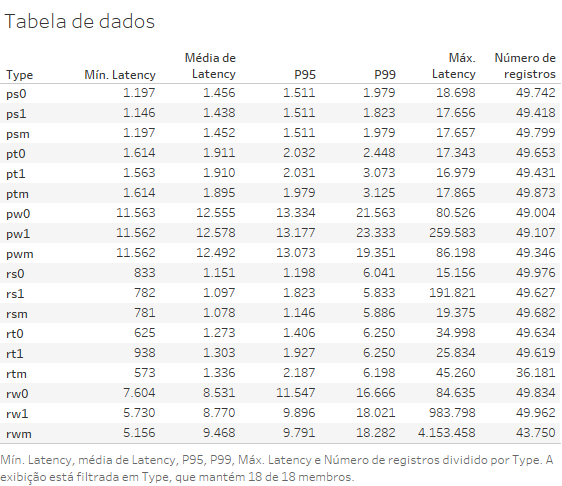
\includegraphics{graficos/Tabeladedados.png}
    \caption{Medições de latência}
    \label{tableau}
\end{figure}

\subsection{Comparativo por kernel}
\subsection{Comparativo por tipo de interrupção}
\subsection{Comparativo por carga de trabalho}
\xchapter{Conclusão}{O que tirei disso}

Fechamento.

Outro parágrafo.

\section{Aprendizados}
\section{Dificuldades}
\section{Pro futuro (?)}
% Importante: Use \xchapter ao inves de \chapter, conforme exemplo abaixo.

%%
%% Parte pos-textual
%%
\backmatter

% Apendices
% Comente se n??o houver ap??ndices
\appendix

% Eh aconselhavel criar cada apendice em um arquivo separado, digamos
% "apendice1.tex", "apendice.tex", ... "apendiceM.tex" e depois
% inclui--los com:
% \include{apendice1}
% \include{apendice2}
% ...
% \include{apendiceM}

% Bibliografia
% ?? aconselh??vel utilizar o BibTeX a partir de um arquivo, digamos "biblio.bib".
% Para ajuda na cria????o do arquivo .bib e utiliza????o do BibTeX, recorra ao
% BibTeXpress em www.cin.ufpe.br/~paguso/bibtexpress
\bibliographystyle{abntex2-alf}
\bibliography{biblio}

% Colofon
% Inclui uma pequena nota com referencia a UFPEThesis
% Comente para omitir
%\colophon

%% Fim do documento
\end{document}
